\section{Лекция 12}

Возмущение \quad $\braupket{\vec{r}_1,~\vec{r}_2}{\hat{V}_{12}}{\psi} = \dfrac{e^2}{r_{12}}\,\psi(\vec{r}_1, \vec{r}_2)$

Для атома гелия решение поставленной задачи с помощью теории возмущений плохо сходится с экспериментом.\\

Построим решение через теорию возмущений:
\[
\Psi^{(0)}(\vec{r}_1, \vec{r}_2) \sim \psi^{(0)}_{n_1 l_1 l_{z_1}}(\vec{r}_1)\,\psi^{(0)}_{n_2 l_2 l_{z_2}}(\vec{r}_2)
\]

рассмотрим энергию одного электрона в водородоподобном ионе:
\[
E^{(0)}_{n_i} = -\frac{Z^2 R_y}{n_i^2}, \qquad R_y = \frac{e^2}{2a_0} \approx 13{,}6 \text{ эВ}
\]
$\Rightarrow$ для двух невзаимодействующих электронов
\[
E^{(0)}_{n_1 n_2} = E^{(0)}_{n_1} + E^{(0)}_{n_2} = -Z^2 R_y\left(\frac{1}{n_1^2} + \frac{1}{n_2^2}\right)
\]

Вспомним, что если мы хотим построить истинную волновую функцию, нужно учесть спины, хоть они и не учитываются в $\hat{H}$: $\xi_i = \{\vec{r}_i,\, s_i\} \implies$ полная функция двух тождественных электронов:
\[
\Psi^{(0)}(\xi_1, \xi_2) = \Psi^{(0)}(\vec{r}_1,\vec{r}_2)\cdot |S,\,S_z,\,s_1 = \tfrac{1}{2},\, s_2 = \tfrac{1}{2}\rangle
\]

По теореме Паули $\Psi^{(0)}(\xi_1, \xi_2) = -\Psi^{(0)}(\xi_2, \xi_1)$, т.е. нужна антисимметричная функция.\\

При сложении двух спинов $\tfrac{1}{2}$ полный вектор состояния $|S{=}0,\,S_z{=}0,\,s_1{=}\tfrac{1}{2},\,s_2{=}\tfrac{1}{2}\rangle = \dfrac{1}{\sqrt{2}}\Big(|{+}^{(1)}\rangle \otimes |{-}^{(2)}\rangle - |{-}^{(1)}\rangle \otimes |{+}^{(2)}\rangle\Big)$ ---
антисимметрично относительно перестановки индексов.\\

Также есть спиновый триплет : $\ket{S=1, S_z = \pm 1}$, $\ket{S=1, S_z = 0}$ --- симметрично.\\

Состояния с максимальными моментами симметричны

$\Rightarrow$ из теоремы Паули:
\[
\underbrace{\Psi^{(0)}(\xi_1,\xi_2)}_{(A)} = \underbrace{\Psi^{(0)}_S(\vec{r}_1,\vec{r}_2)}_{(S)} \cdot \underbrace{|S{=}0,\,S_z{=}0\rangle}_{(A)}
\]
или
\[
\underbrace{\Psi^{(0)}(\xi_1,\xi_2)}_{(A)} = \underbrace{\Psi^{(0)}_A(\vec{r}_1,\vec{r}_2)}_{(A)} \cdot \underbrace{|S{=}1,\,S_z\rangle}_{(S)}
\]

\subsection{\S XVII.4.2. Атом гелия. Основное состояние.}

\[
n_1 = n_2 = 1, \quad l_1 = l_2 = 0 \implies l_{z_1} = l_{z_2} = 0 \qquad \text{--- $1s^2$-конфигурация}
\]

У нас есть $\Psi^{(0)}_{100}(\vec{r}) = \sqrt{\dfrac{Z^3}{\pi a_0^3}}\,e^{-Zr/a_0}$
$\implies$
$\Psi^{(0)}_S(\vec{r}_1, \vec{r}_2) = \Psi^{(0)}_{100}(\vec{r}_1)\,\Psi^{(0)}_{100}(\vec{r}_2)$, \quad $\Psi^{(0)}_A$ \text{не существует}.\\

$\Rightarrow$ в основном состоянии атома He 2 электрона могут находиться только в состоянии спинового синглета (предположение).\\


Найдём поправку \quad $E^{(1)}_{n_1=n_2=1} = \langle\Psi^{(0)}|\hat{V}|\Psi^{(0)}\rangle = \langle\Psi^{(0)}_S|\hat{V}_{12}|\Psi^{(0)}_S\rangle\cdot\langle s_1, s_2|\hat{1}|s_1,s_2\rangle = $
\[
 = \int d\vec{r}_1\,d\vec{r}_2\;\Psi^{(0)*}_{100}(\vec{r}_1)\,\Psi^{(0)*}_{100}(\vec{r}_2)\;\dfrac{e^2}{|\vec{r}_1-\vec{r}_2|}\;\underbrace{\Psi^{(0)}_{100}(\vec{r}_2)\,\Psi^{(0)}_{100}(\vec{r}_1)}_{\mathbb{R}} =
\]

\[
= \int d\vec{r}_1\,d\vec{r}_2\;|\Psi^{(0)}_{100}(\vec{r}_1)|^2\,|\Psi^{(0)}_{100}(\vec{r}_2)|^2\;\frac{e^2}{|\vec{r}_1-\vec{r}_2|}
= \frac{5}{4}\,Z R_y, \qquad Z = 2
\]

\[
E_{n_1=n_2=1} = E^{(0)}_{n_1=n_2=1} + E^{(1)}_{n_1=n_2=1}
= (-8 + \frac{5}{2})\,R_y = -\frac{11}{2}\,R_y = -\frac{11}{4}\,E_h = -2{,}75\,E_h,
\]
где $E_h$ --- атомная единица энергии.

Эксперимент: $E_{n_1=n_2=1} \approx -2{,}9\,E_h$. Плохое согласие с точным значением атомных чисел.

\subsection{\S XVII.4.3. Атом гелия. Возбуждённое состояние. Обменная энергия.}

У 1 из электронов в основном состоянии \quad $n = 1$, $l = 0$, $l_z = 0$,
а другой в возбужденном $S$-состоянии \quad $n = 2$, $l = 0$, $l_z = 0$.

Теперь можно построить и $\Psi^{(0)}_S$, и $\Psi^{(0)}_A$.

\[
\Psi^{(0)}_S(\vec{r}_1, \vec{r}_2) = \frac{1}{\sqrt{2}}\Big(\Psi^{(0)}_{100}(\vec{r}_1)\,\Psi^{(0)}_{200}(\vec{r}_2) + \Psi^{(0)}_{200}(\vec{r}_1)\,\Psi^{(0)}_{100}(\vec{r}_2)\Big)
\]
\[
\Psi^{(0)}_A(\vec{r}_1, \vec{r}_2) = \frac{1}{\sqrt{2}}\Big(\Psi^{(0)}_{100}(\vec{r}_1)\,\Psi^{(0)}_{200}(\vec{r}_2) - \Psi^{(0)}_{200}(\vec{r}_1)\,\Psi^{(0)}_{100}(\vec{r}_2)\Big)
\]

\[
E^{(0)}_{1,\,2} = -Z^2 R_y\left(\frac{1}{1} + \frac{1}{4}\right) = -\frac{5}{4}\,Z^2 R_y = -5\,R_y
\]

Поправка \quad $E^{(1)}_{1,2} = \displaystyle\int d\vec{r}_1\,d\vec{r}_2\;\Big|\Psi^{(0)}_{S(A)}(\vec{r}_1,\vec{r}_2)\Big|^2\,\dfrac{e^2}{|\vec{r}_1-\vec{r}_2|}$
\[
= \frac{1}{2}\int d\vec{r}_1\,d\vec{r}_2\;\Big|\Psi^{(0)}_{100}(\vec{r}_1)\,\Psi^{(0)}_{200}(\vec{r}_2) \pm \Psi^{(0)}_{200}(\vec{r}_1)\,\Psi^{(0)}_{100}(\vec{r}_2)\Big|^2\,\frac{e^2}{|\vec{r}_1-\vec{r}_2|}
= C \pm A,
\]
где С и А --- интегралы вида:

\begin{align*}
	C &= \int d\vec{r}_1\,d\vec{r}_2\;\big|\Psi^{(0)}_{100}(\vec{r}_1)\big|^2\,\big|\Psi^{(0)}_{200}(\vec{r}_2)\big|^2\,\frac{e^2}{|\vec{r}_1-\vec{r}_2|}
	\qquad\text{--- кулоновский интеграл, очевидно $C > 0$}\\[6pt]
	A &= \int d\vec{r}_1\,d\vec{r}_2\;\Psi^{(0)}_{100}(\vec{r}_1)\,\Psi^{(0)}_{200}(\vec{r}_2)\,\Psi^{(0)*}_{200}(\vec{r}_1)\,\Psi^{(0)*}_{100}(\vec{r}_2)\,\frac{e^2}{|\vec{r}_1-\vec{r}_2|}
\end{align*}
--- обменный интеграл, возникает за счёт интерференции (или интеграл обменного взаимодействия).

Докажем, что $A > 0$.\\

Введём $\varphi(\vec{r}_1) = \displaystyle\int d\vec{r}_2\;\dfrac{\rho(\vec{r}_2)}{|\vec{r}_1 - \vec{r}_2|}$, где $\rho(\vec{r}_2) = e\,\Psi^{(0)*}_{100}(\vec{r}_2)\,\Psi^{(0)}_{200}(\vec{r}_2)$
$\implies \varphi(\vec{r}_1)$ --- кулоновский потенциал $\Rightarrow$ удовлетворяет уравнению Пуассона:
\[
\Delta\varphi(\vec{r}) = -4\pi\rho(\vec{r})
\]

$\Rightarrow A = \displaystyle\int d\vec{r}_1\;\varphi(\vec{r}_1)\,\rho^*(\vec{r}_1) = -\dfrac{1}{4\pi}\int d\vec{r}_1\;\varphi(\vec{r}_1)\,(\Delta\varphi(\vec{r}_1))^* = \text{ на бесконечности }\;\Psi \to 0$ = 
$\displaystyle\frac{1}{4\pi}\int d\vec{r}_1\;|\vec{\nabla}\varphi(\vec{r}_1)|^2 \geq 0$ \quad ч.т.д.\\

Стало $E_{S(A)} = E^{(0)}_{1,2} + E^{(1)}_{S(A)} = -5\,R_y + C \pm A$.

\begin{figure}[H]
	\centering
	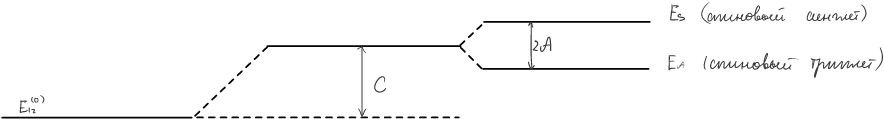
\includegraphics[width=0.9\linewidth]{images/l12_1.jpg}
\end{figure}

Это расщепление называется обменным взаимодействием (эл.-эл. взаимодействие, не имеет классического аналога).

\bigskip


\section{XVIII. Квантование свободного электромагнитного поля и элементы теории излучения}

\subsection{\S XVIII.1. Описание свободного классического электромагнитного поля в вакууме.}

Напряжённость электрического поля $\vec{\mathcal{E}}(\vec{r},t)$, магнитного $\vec{\mathcal{H}}(\vec{r},t)$.\\

Введём потенциалы: $\varphi(\vec{r},t)$, $\vec{A}(\vec{r},t)$. Они таковы, что
\[
\vec{\mathcal{E}}(\vec{r},t) = -\nabla\varphi(\vec{r},t) - \frac{1}{c}\frac{\partial}{\partial t}\vec{A}(\vec{r},t), \qquad
\vec{\mathcal{H}}(\vec{r},t) = \mathrm{rot}\,\vec{A}(\vec{r},t) = \bigl[\vec{\nabla}\times\vec{A}(\vec{r},t)\bigr]
\]

\[
\begin{cases}
	\bigl[\vec{\nabla}\times\vec{\mathcal{H}}\bigr] = \dfrac{1}{c}\,\dfrac{\partial\vec{\mathcal{E}}}{\partial t}\\[6pt]
	\bigl[\vec{\nabla}\times\vec{\mathcal{E}}\bigr] = -\dfrac{1}{c}\,\dfrac{\partial\vec{\mathcal{H}}}{\partial t}\\[6pt]
	(\vec{\nabla}\vec{\mathcal{E}}) = 0 \qquad \text{т.к. свободные заряды}\\[4pt]
	(\vec{\nabla}\vec{\mathcal{H}}) = 0 \qquad \text{по построению}
\end{cases}
\qquad\text{--- уравнения Максвелла}
\]

На все поле наложим кулоновскую калибровку: $\mathrm{div}\,\vec{A} = (\vec{\nabla}\vec{A}) = 0$.\\
Вспомним про калибровочное преобразование:
\[
\begin{cases}
	\vec{A}' = \vec{A} + \nabla f\\[4pt]
	\varphi' = \varphi - \dfrac{1}{c}\,\dfrac{\partial f}{\partial t}
\end{cases}
\]

Из кулоновской калибровки, выберем $f$ так, что $\varphi(\vec{r},t) = 0$. Тогда
\[
\vec{\mathcal{H}} = \mathrm{rot}\,\vec{A}, \qquad \vec{\mathcal{E}} = -\frac{1}{c}\,\frac{\partial\vec{A}}{\partial t}
\]

Из уравнений Максвелла $\Rightarrow \Delta\vec{A} - \dfrac{1}{c^2}\,\dfrac{\partial^2}{\partial t^2}\vec{A} = \vec{0}$ \quad или \quad $\Box\,\vec{A} = \vec{0}$ \quad --- уравнение Даламбера, найдём общее решение.

Поместим поле в ящик объёмом $V = L^3$ (для упрощения нормировки).

Частные положительно-частотное:
\[
A^{(+)}(\vec{k},\lambda) = N_k\,C_{\vec{k},\lambda}\;{\vec{e}(\vec{k},\lambda)}\;e^{-i(\omega_k t - \vec{k}\vec{r})}
\]
Подставим в уравнение $\Rightarrow \omega_k^2 = c^2 k^2$ --- \textbf{закон дисперсии}.

\[
A^{(-)}(\vec{k},\lambda) = N_k\,\tilde{C}_{\vec{k},\lambda}\;\tilde{\vec{e}}(\vec{k},\lambda)\;e^{+i(\omega_k t - \vec{k}\vec{r})} \quad\text{--- получили тот же з-н дисперсии}
\]

Из эксперимента фотон имеет две поляризации: $\lambda = 1$ и $\lambda = 2$ (обозначения).

Потребуем: $\vec{e}^*(\vec{k},\lambda)\,\vec{e}(\vec{k},\lambda') = \delta_{\lambda\lambda'}$.

Из кулоновской калибровки:
\[
\begin{cases}
	\mathrm{div}\,\vec{A}^{(+)}(\vec{k},\lambda) = 0\\
	\mathrm{div}\,\vec{A}^{(-)}(\vec{k},\lambda) = 0
\end{cases}
\implies
\begin{cases}
	(\vec{e}(\vec{k},\lambda),\,\vec{k}) = 0\\
	(\tilde{\vec{e}}(\vec{k},\lambda),\,\vec{k}) = 0
\end{cases}
\]

$\Rightarrow$ общее решение уравнения Даламбера:
\[
\vec{A}(\vec{r},t) = \sum_{\lambda=1}^{2}\sum_{\vec{k}} N_k\Bigl(C_{\vec{k}\lambda}\;\vec{e}(\vec{k},\lambda)\,e^{-i(\omega_k t - \vec{k}\vec{r})} + \tilde{C}_{\vec{k}\lambda}\;\tilde{\vec{e}}(\vec{k},\lambda)\,e^{+i(\omega_k t - \vec{k}\vec{r})}\Bigr)
\]

$\vec{\mathcal{E}}$ и $\vec{\mathcal{H}}$ --- действ. функции $\Rightarrow \vec{A}^*$ --- действ. функция $\Rightarrow \vec{A}^*(\vec{r},t) = \vec{A}(\vec{r},t)$
$\Rightarrow$
$\begin{cases}
	\tilde{\vec{e}}(\vec{k},\lambda) = \vec{e}^*(\vec{k},\lambda)\\[4pt]
	\tilde{C}_{\vec{k}\lambda} = C_{\vec{k}\lambda}^* = C_{\vec{k}\lambda}^\dagger
\end{cases}$

Для простоты поляризации линейные $\Rightarrow \tilde{\vec{e}} = \vec{e}$

\[
\Rightarrow \vec{A}(\vec{r},t) = \sum_{\lambda=1}^{2}\sum_{\vec{k}} N_k\;\vec{e}(\vec{k},\lambda)\Bigl(C_{\vec{k}\lambda}\,e^{-i(\omega_k t - \vec{k}\vec{r})} + C^\dagger_{\vec{k}\lambda}\,e^{+i(\omega_k t - \vec{k}\vec{r})}\Bigr)
\]

\[
\Rightarrow \vec{\mathcal{E}}(\vec{r},t) = -\frac{1}{c}\,\frac{\partial\vec{A}}{\partial t}
= \frac{i}{c}\sum_{\lambda=1}^{2}\sum_{\vec{k}} N_k\;\vec{e}(\vec{k},\lambda)\,\omega_k\Bigl(C_{\vec{k}\lambda}\,e^{-i(\omega_k t - \vec{k}\vec{r})} - C^\dagger_{\vec{k}\lambda}\,e^{+i(\omega_k t - \vec{k}\vec{r})}\Bigr)
\]

\[
\vec{\mathcal{H}}(\vec{r},t) = \bigl[\vec{\nabla}\times\vec{A}\bigr]
= i\sum_{\lambda=1}^{2}\sum_{\vec{k}} N_k\;\bigl[\vec{k}\times\vec{e}(\vec{k},\lambda)\bigr]\Bigl(C_{\vec{k}\lambda}\,e^{-i(\omega_k t - \vec{k}\vec{r})} - C^\dagger_{\vec{k}\lambda}\,e^{+i(\omega_k t - \vec{k}\vec{r})}\Bigr)
\]

\subsection{\S XVIII.2. Квантование свободного электро-магнитного поля.}

Каждому классическому осциллятору поставим в соответствие квантовый осциллятор (той же частоты).\\

Посчитаем энергию поля двумя сособами:
\begin{enumerate}
	\item $E = \dfrac{1}{8\pi}\displaystyle\int\limits_V d\vec{r}\;\Bigl(\vec{\mathcal{E}}^2 + \vec{\mathcal{H}}^2\Bigr)$
	\item сумма энергий квантовых осцилляторов
\end{enumerate}

Потом сопоставим и найдём константы.